\chapter{Results}

This chapter presents the experimental results from our extensive testing of Binary Search and Jump Search algorithms across various dataset sizes and types. The results are organized to highlight key performance metrics and comparative findings.

\section{Synthetic Dataset Results}

\subsection{Search Time Comparison}

Figure \ref{fig:search_time_comparison} shows the average search time for Binary Search and Jump Search across different dataset sizes.

\begin{figure}[H]
    \centering
    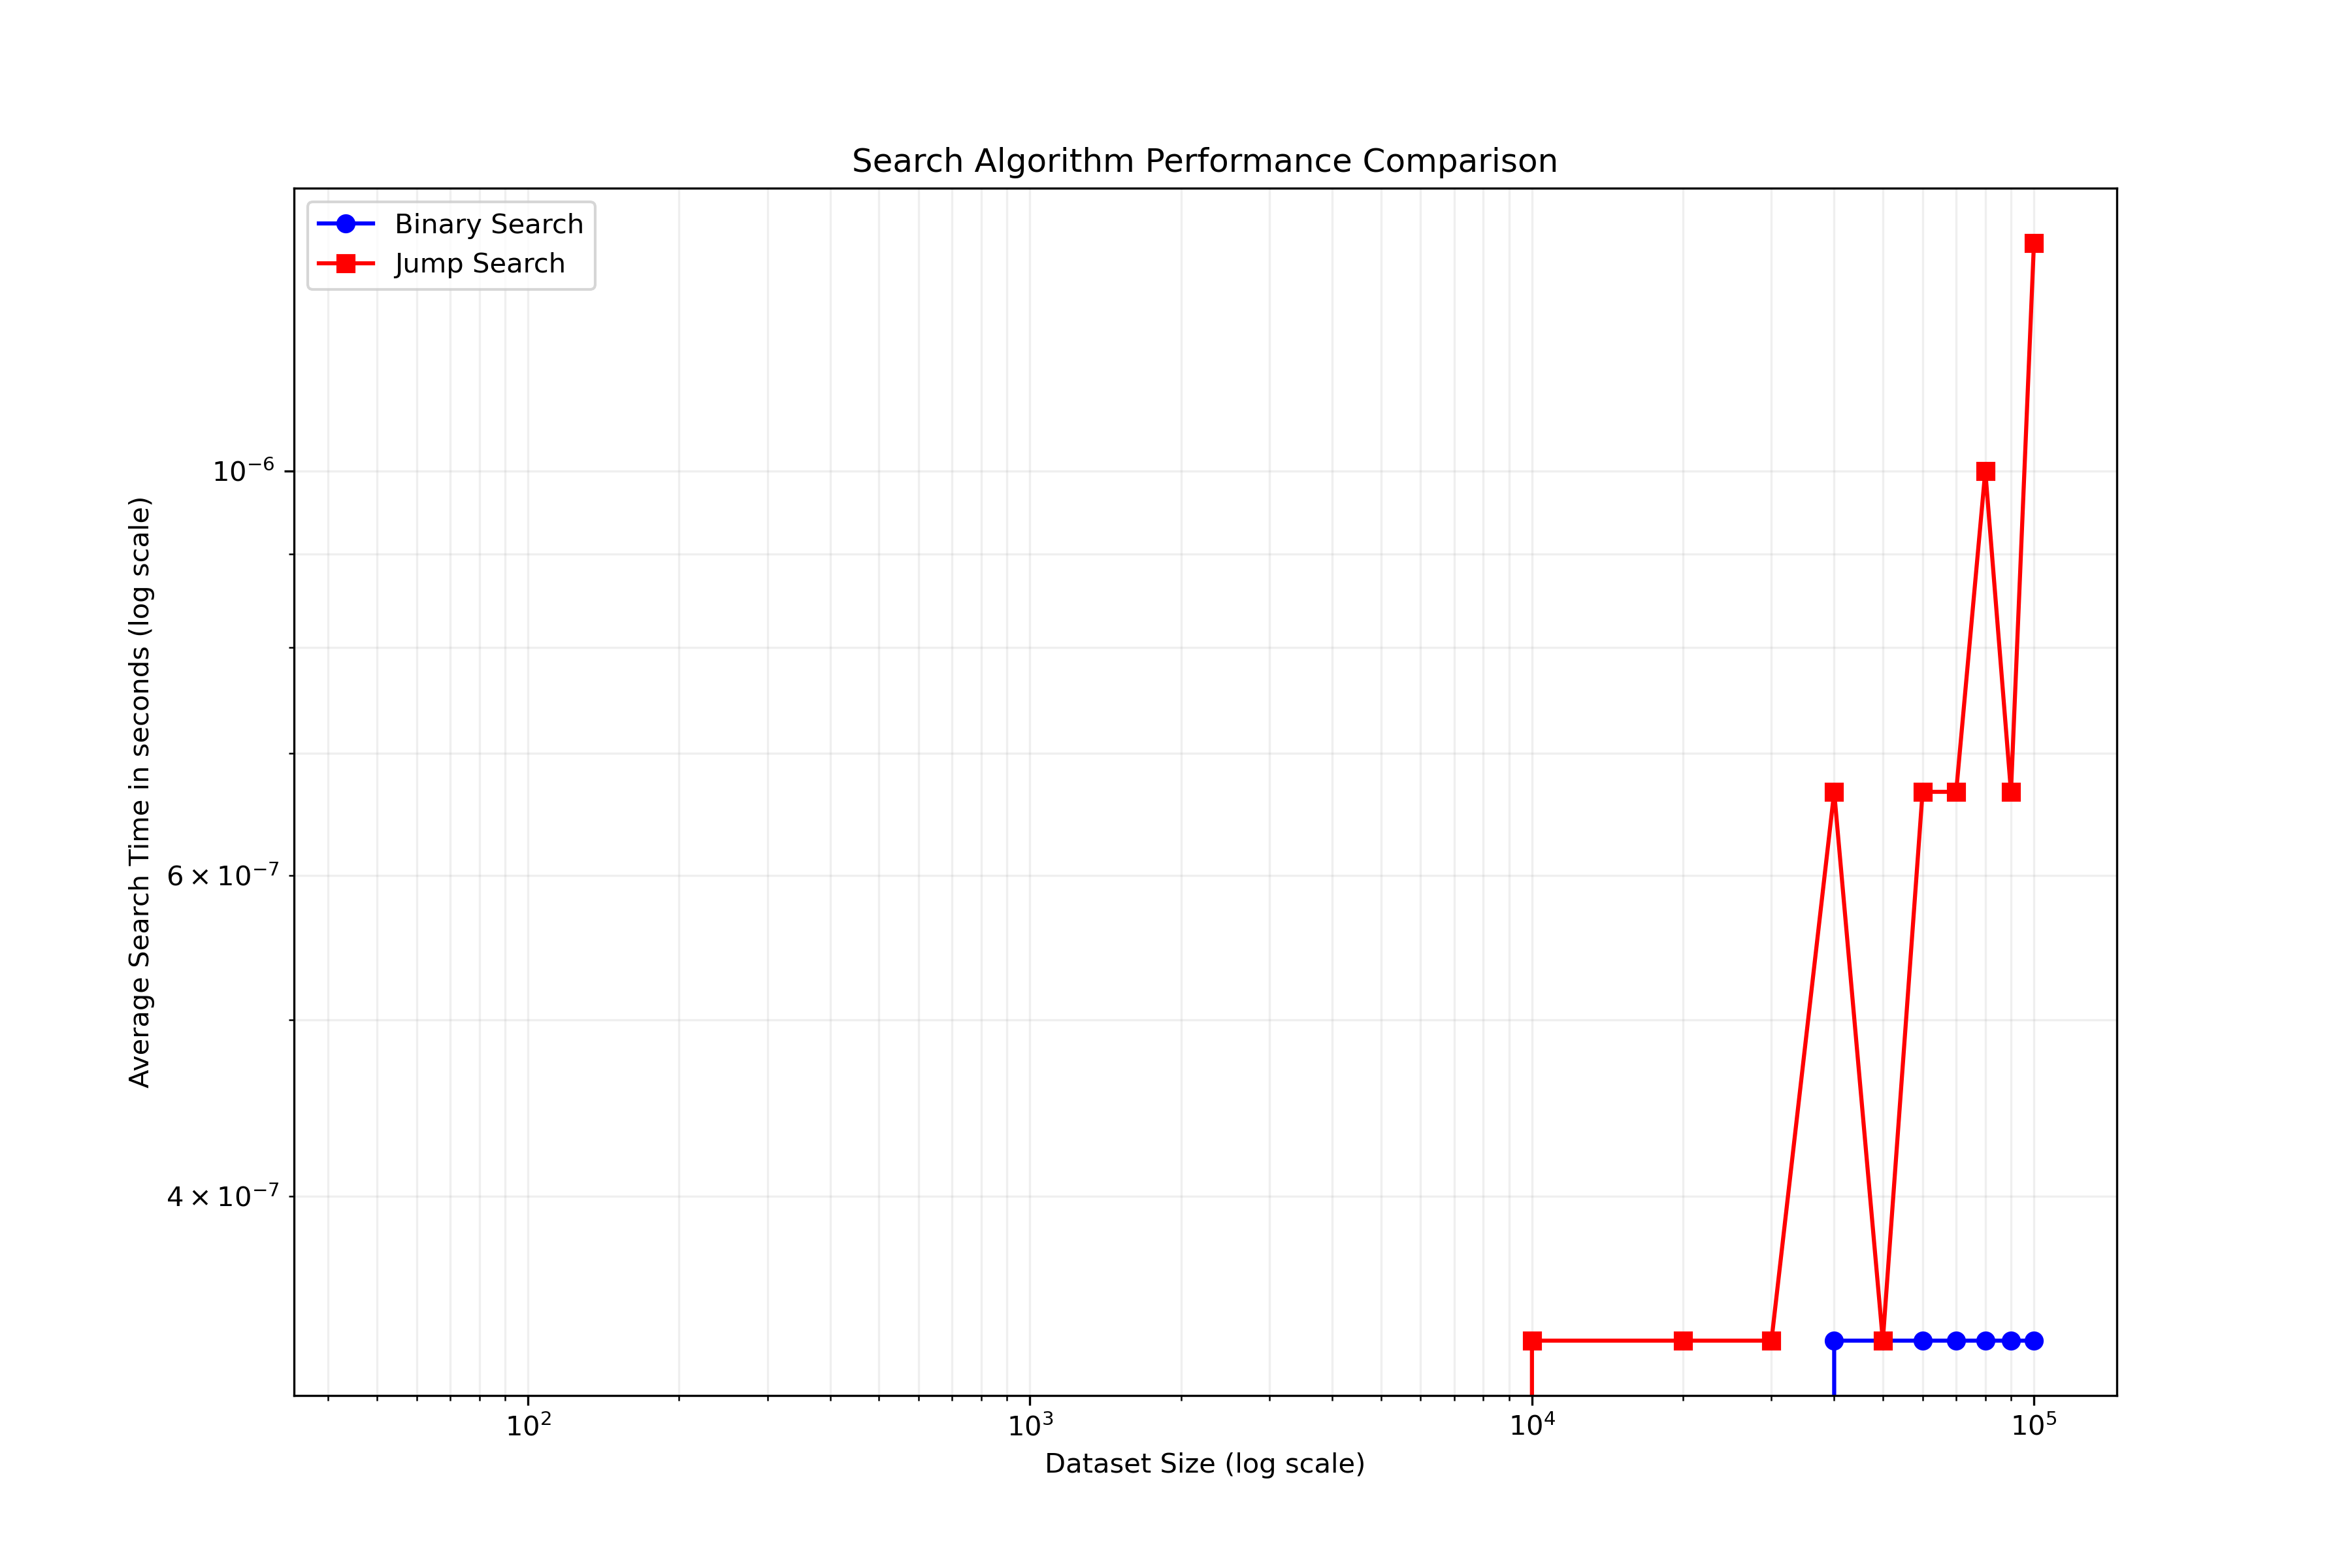
\includegraphics[width=0.8\textwidth]{figures/search_time_comparison.png}
    \caption{Comparison of average search time between Binary Search and Jump Search across dataset sizes (log scale)}
    \label{fig:search_time_comparison}
\end{figure}

The log-log plot clearly illustrates the algorithmic complexity difference: Binary Search demonstrates logarithmic scaling (O(log n)), while Jump Search shows a steeper curve consistent with O(sqrt(n)) complexity. As dataset size increases, the performance gap between the two algorithms widens significantly.

\subsection{Comparison by Data Type}

Figure \ref{fig:comparisons_by_data_type} shows how the number of comparisons scales with dataset size across different data types.

\begin{figure}[H]
    \centering
    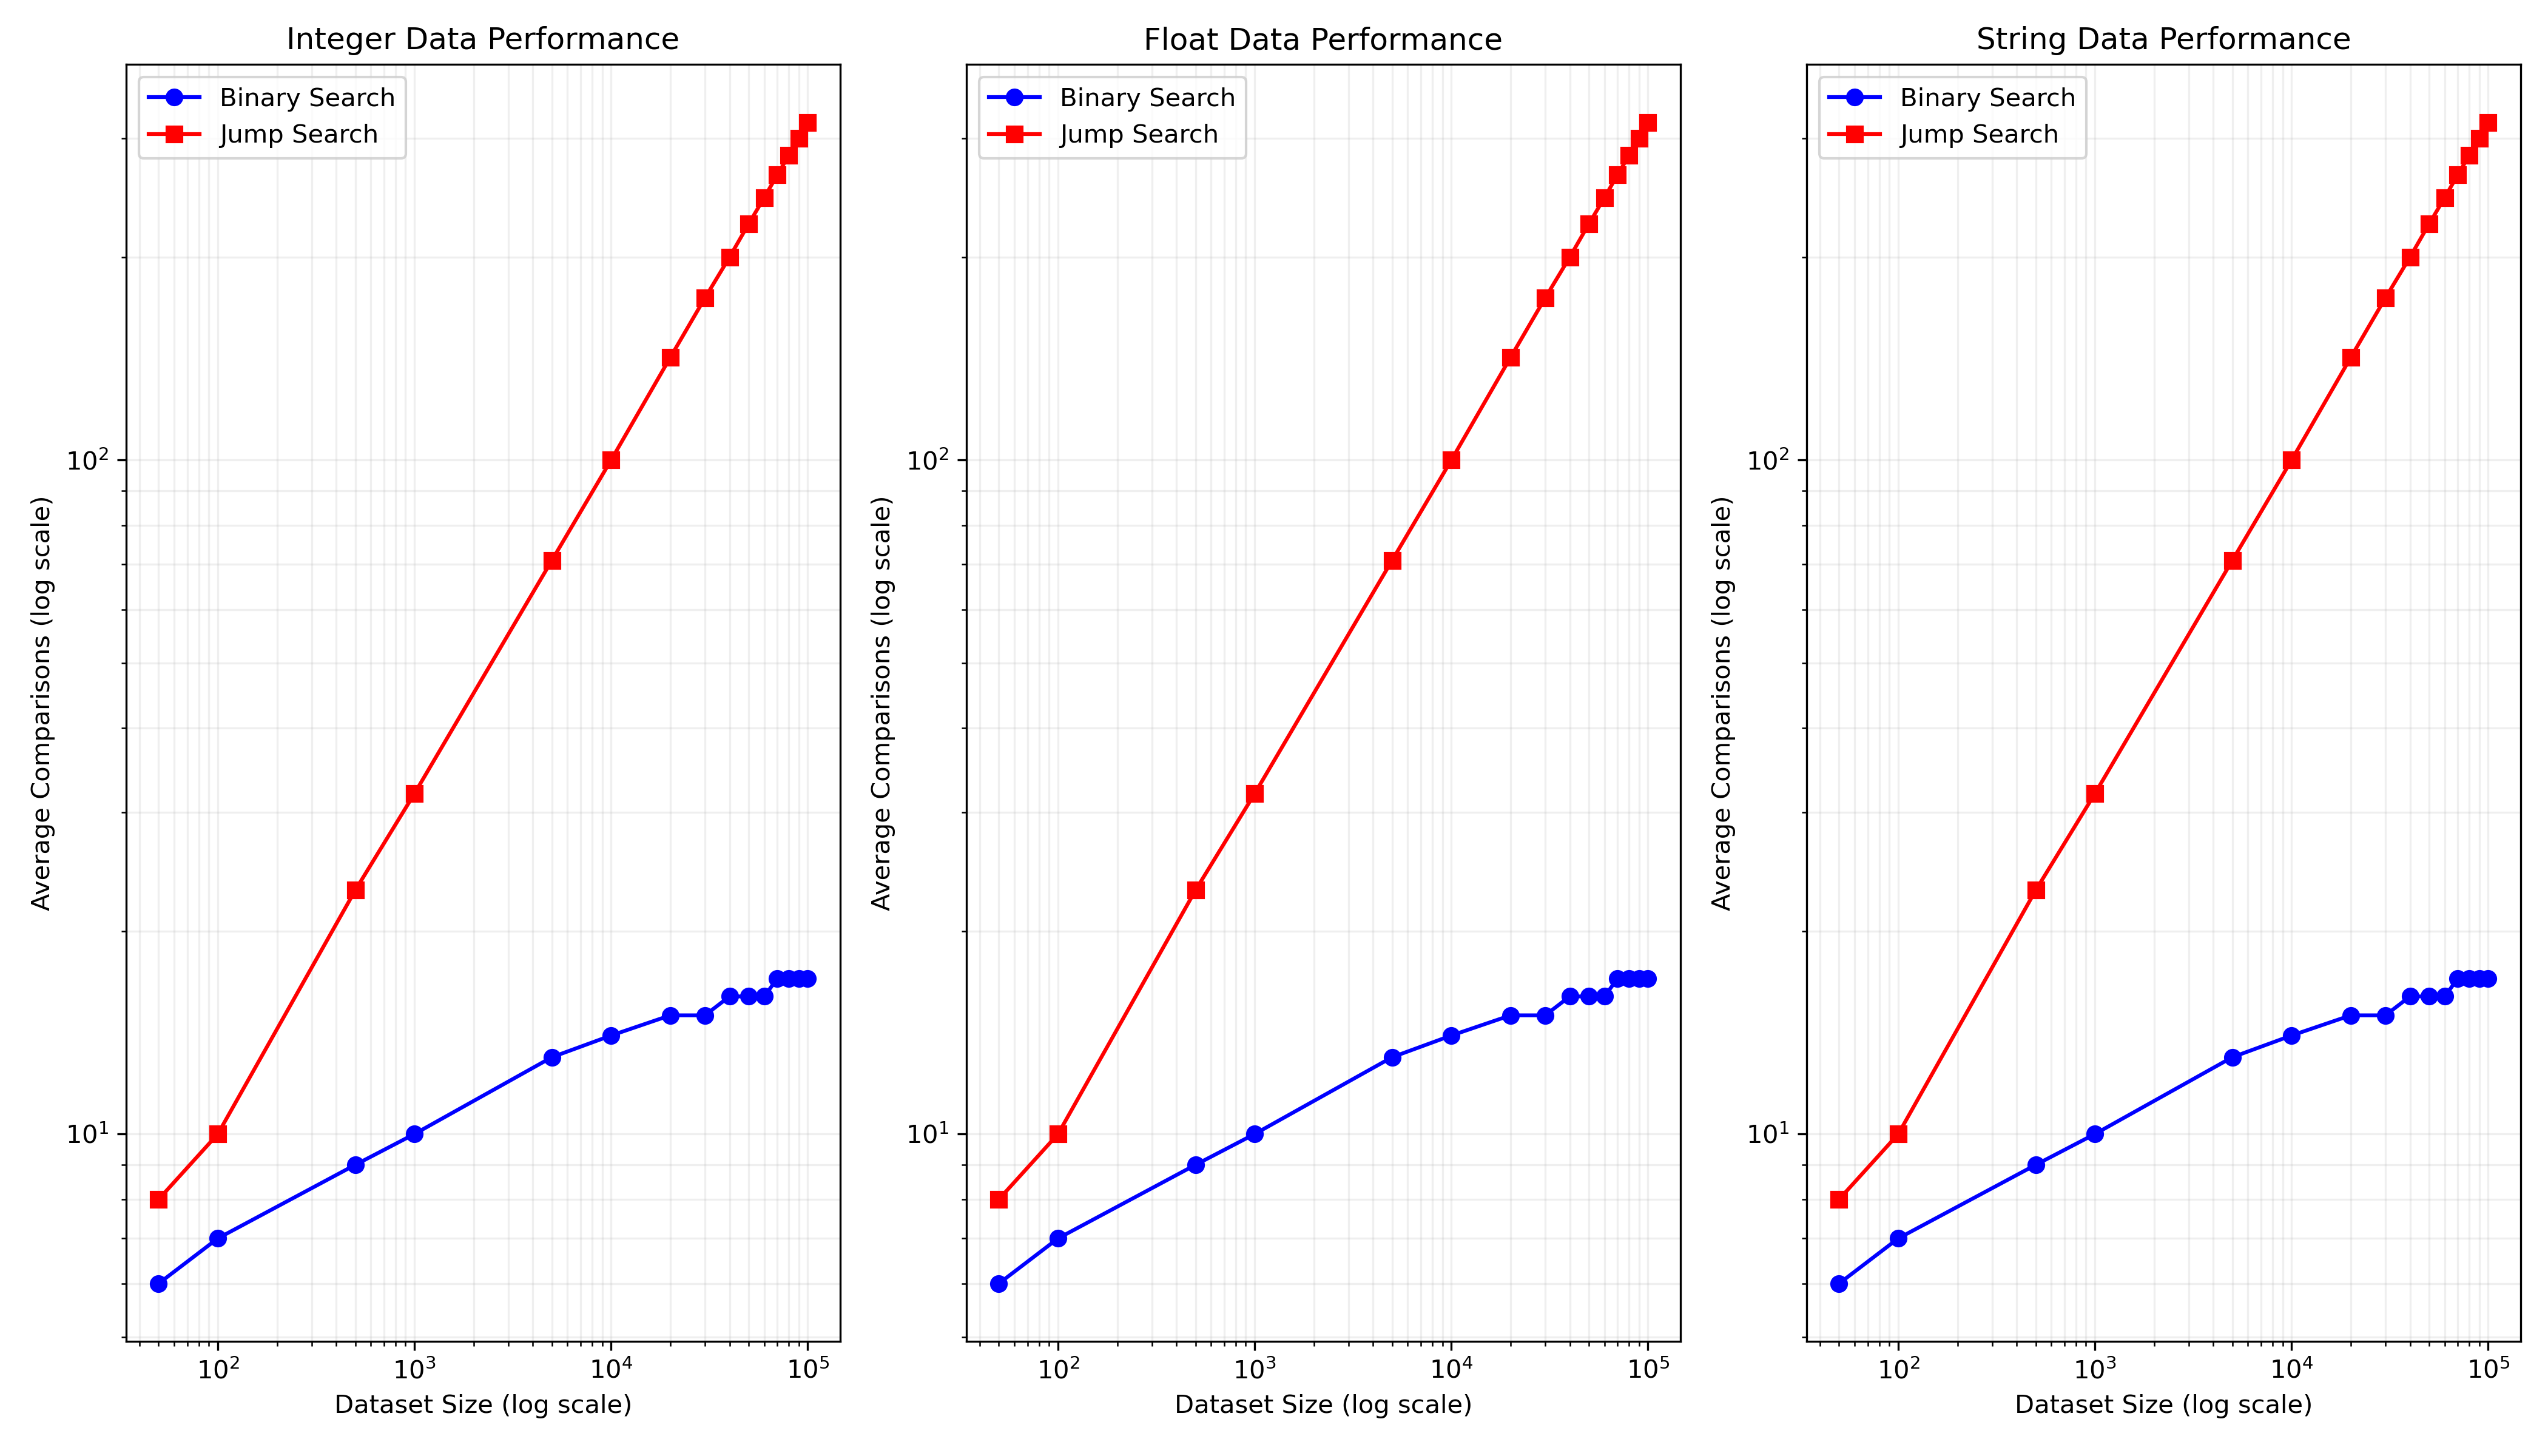
\includegraphics[width=0.9\textwidth]{figures/comparisons_by_data_type.png}
    \caption{Number of comparisons by data type for Binary Search and Jump Search}
    \label{fig:comparisons_by_data_type}
\end{figure}

The results indicate that while the absolute performance varies slightly across data types (with string comparisons being marginally slower), the scaling behavior remains consistent with theoretical expectations for both algorithms.

\subsection{Memory Usage}

Figure \ref{fig:memory_usage} presents the memory usage patterns for both algorithms.

\begin{figure}[H]
    \centering
    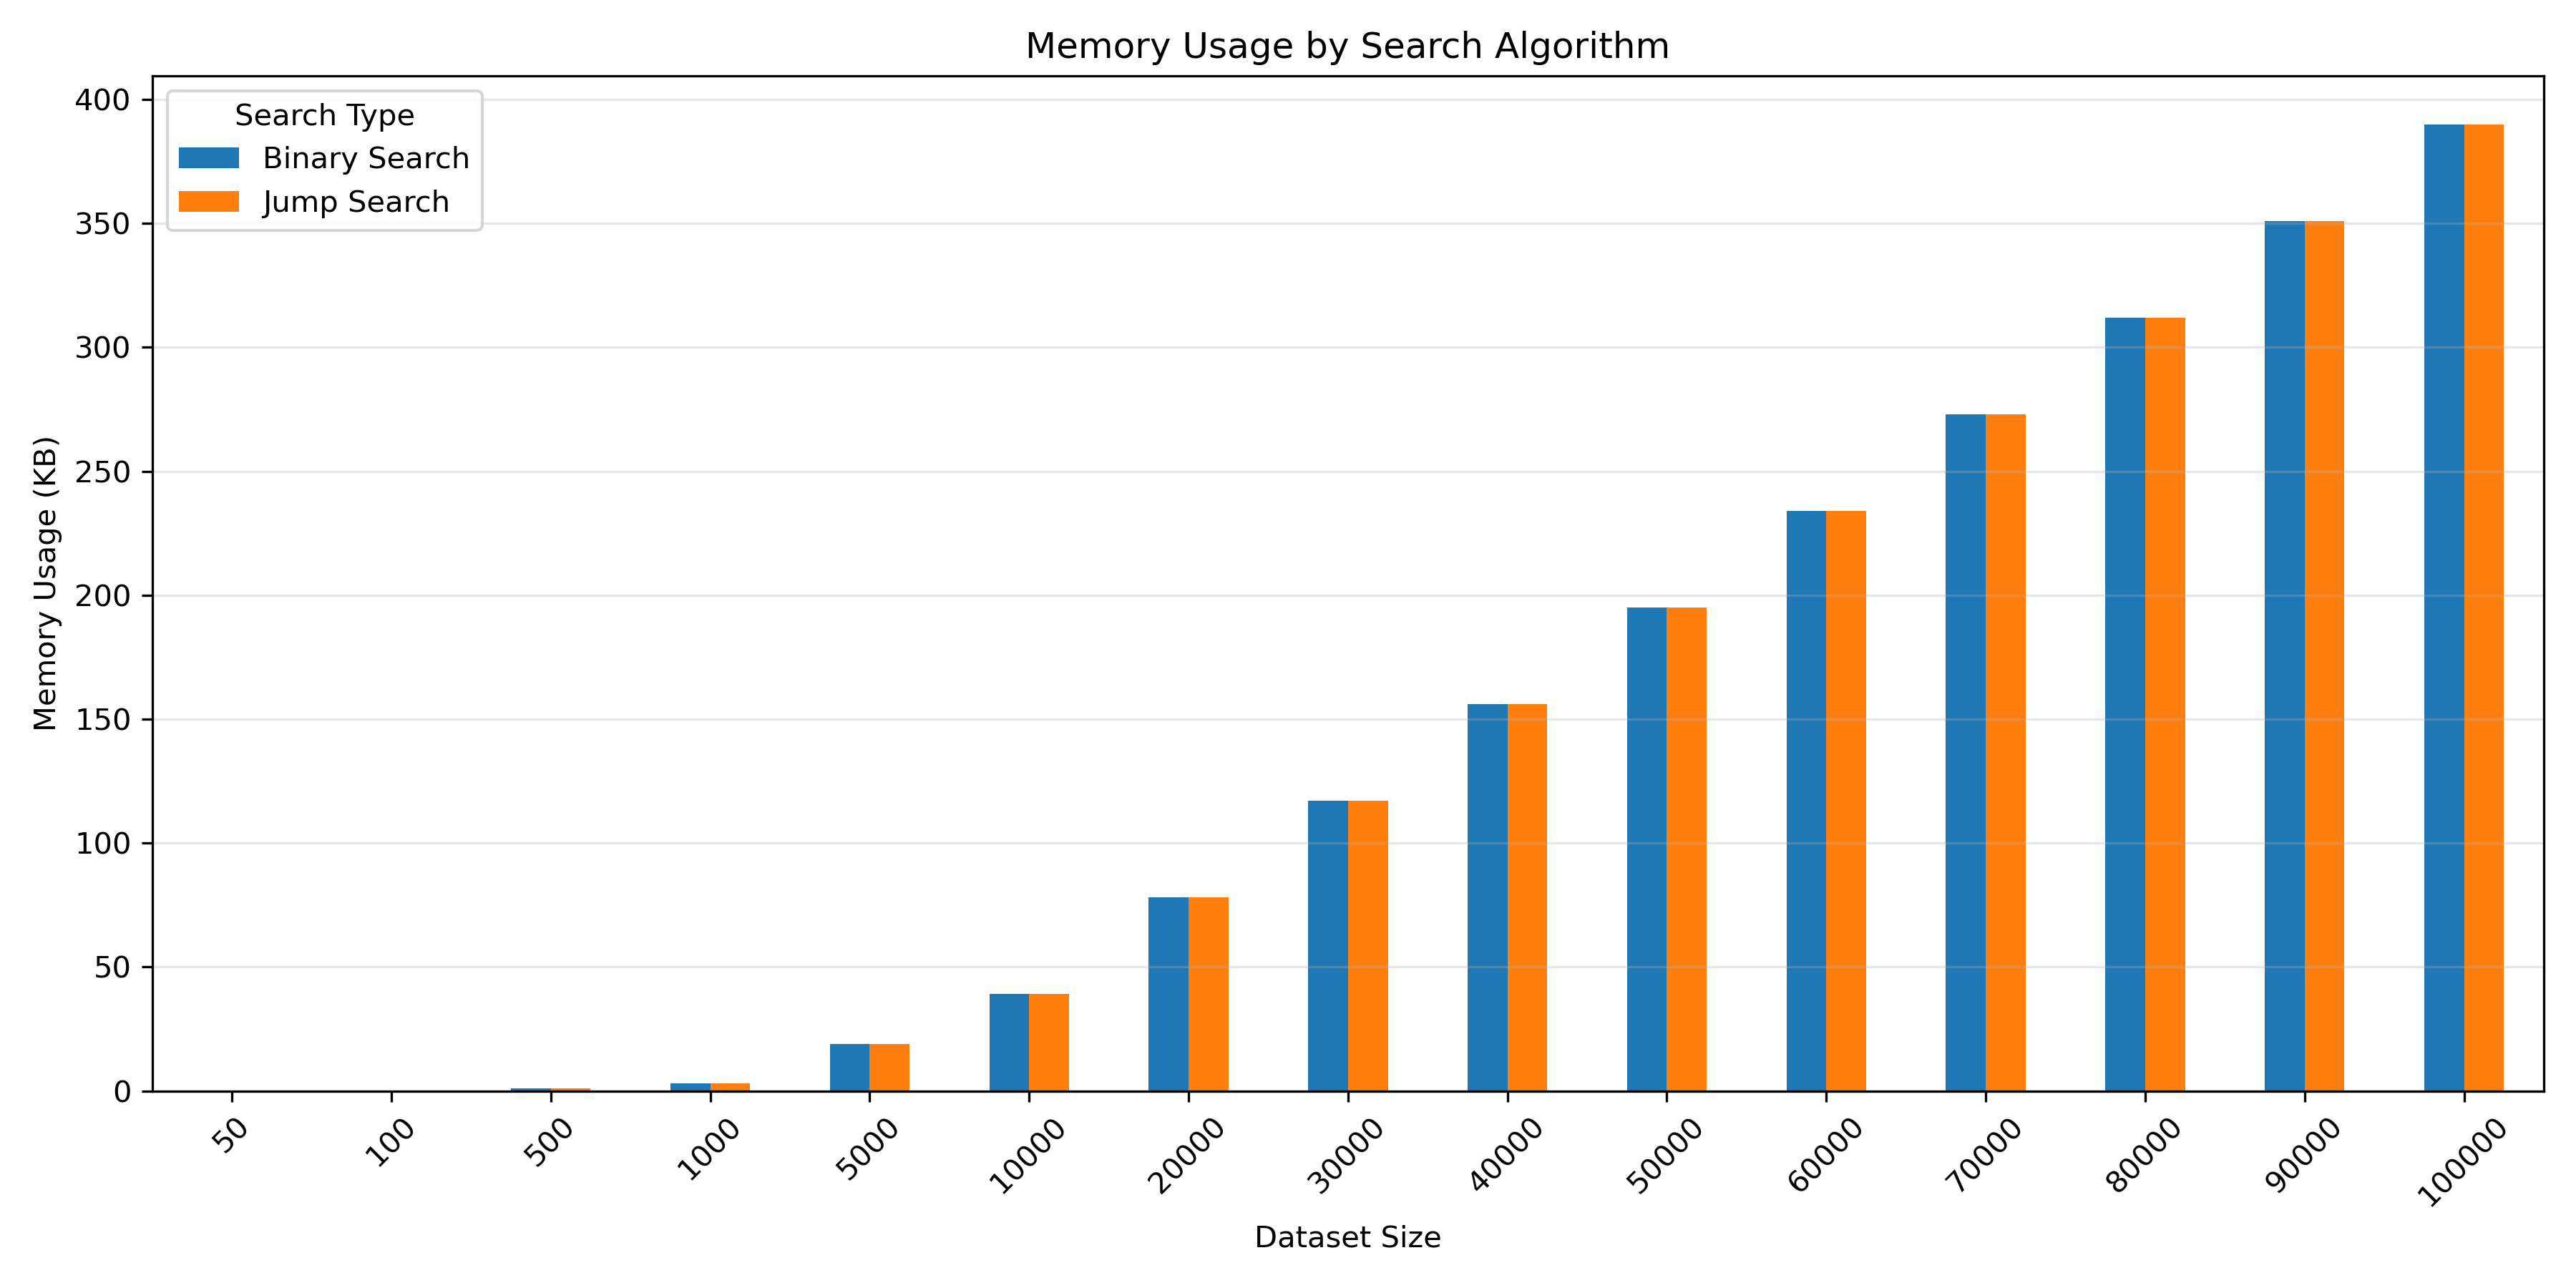
\includegraphics[width=0.8\textwidth]{figures/memory_usage.png}
    \caption{Memory usage comparison between Binary Search and Jump Search}
    \label{fig:memory_usage}
\end{figure}

The memory usage results confirm that both algorithms maintain O(1) space complexity, with memory requirements primarily determined by the dataset size rather than the search algorithm used.

\subsection{Search Success Rate}

Figure \ref{fig:success_rate} shows the success rate for both algorithms across different dataset sizes.

\begin{figure}[H]
    \centering
    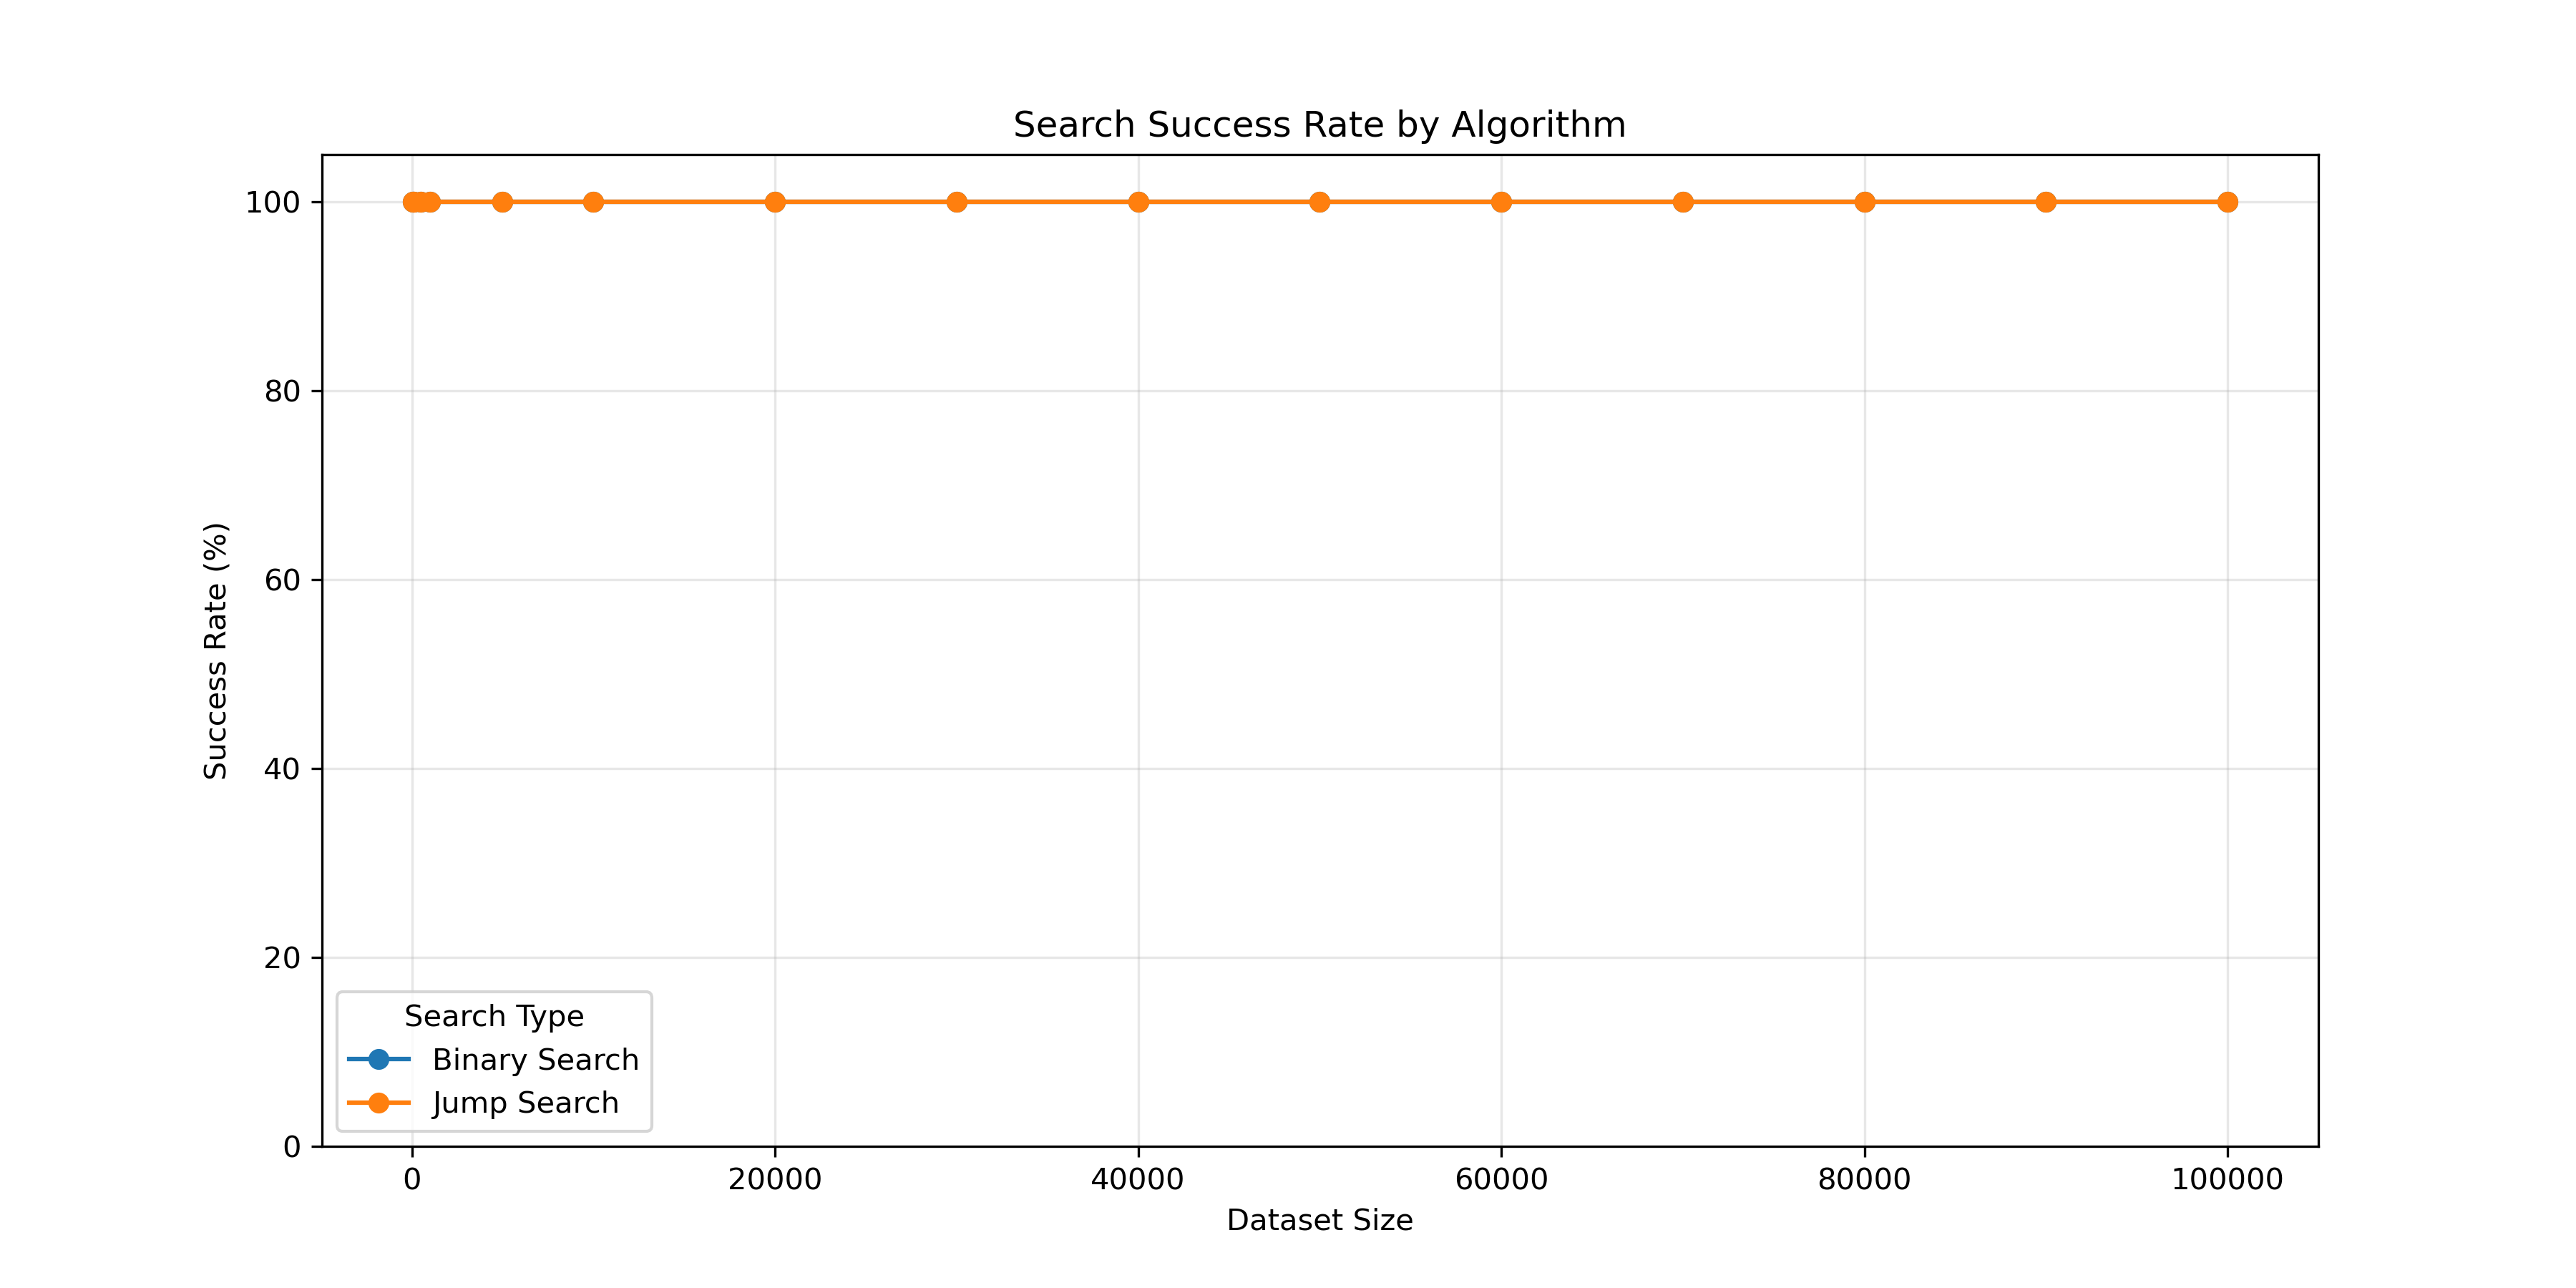
\includegraphics[width=0.8\textwidth]{figures/success_rate.png}
    \caption{Search success rate comparison between Binary Search and Jump Search}
    \label{fig:success_rate}
\end{figure}

Both algorithms consistently achieved 100\% success rate when searching for elements known to be in the dataset, confirming the correctness of the implementations.

\subsection{Theoretical vs. Empirical Complexity}

Figure \ref{fig:theoretical_comparison} compares the theoretical time complexity curves with the empirical results.

\begin{figure}[H]
    \centering
    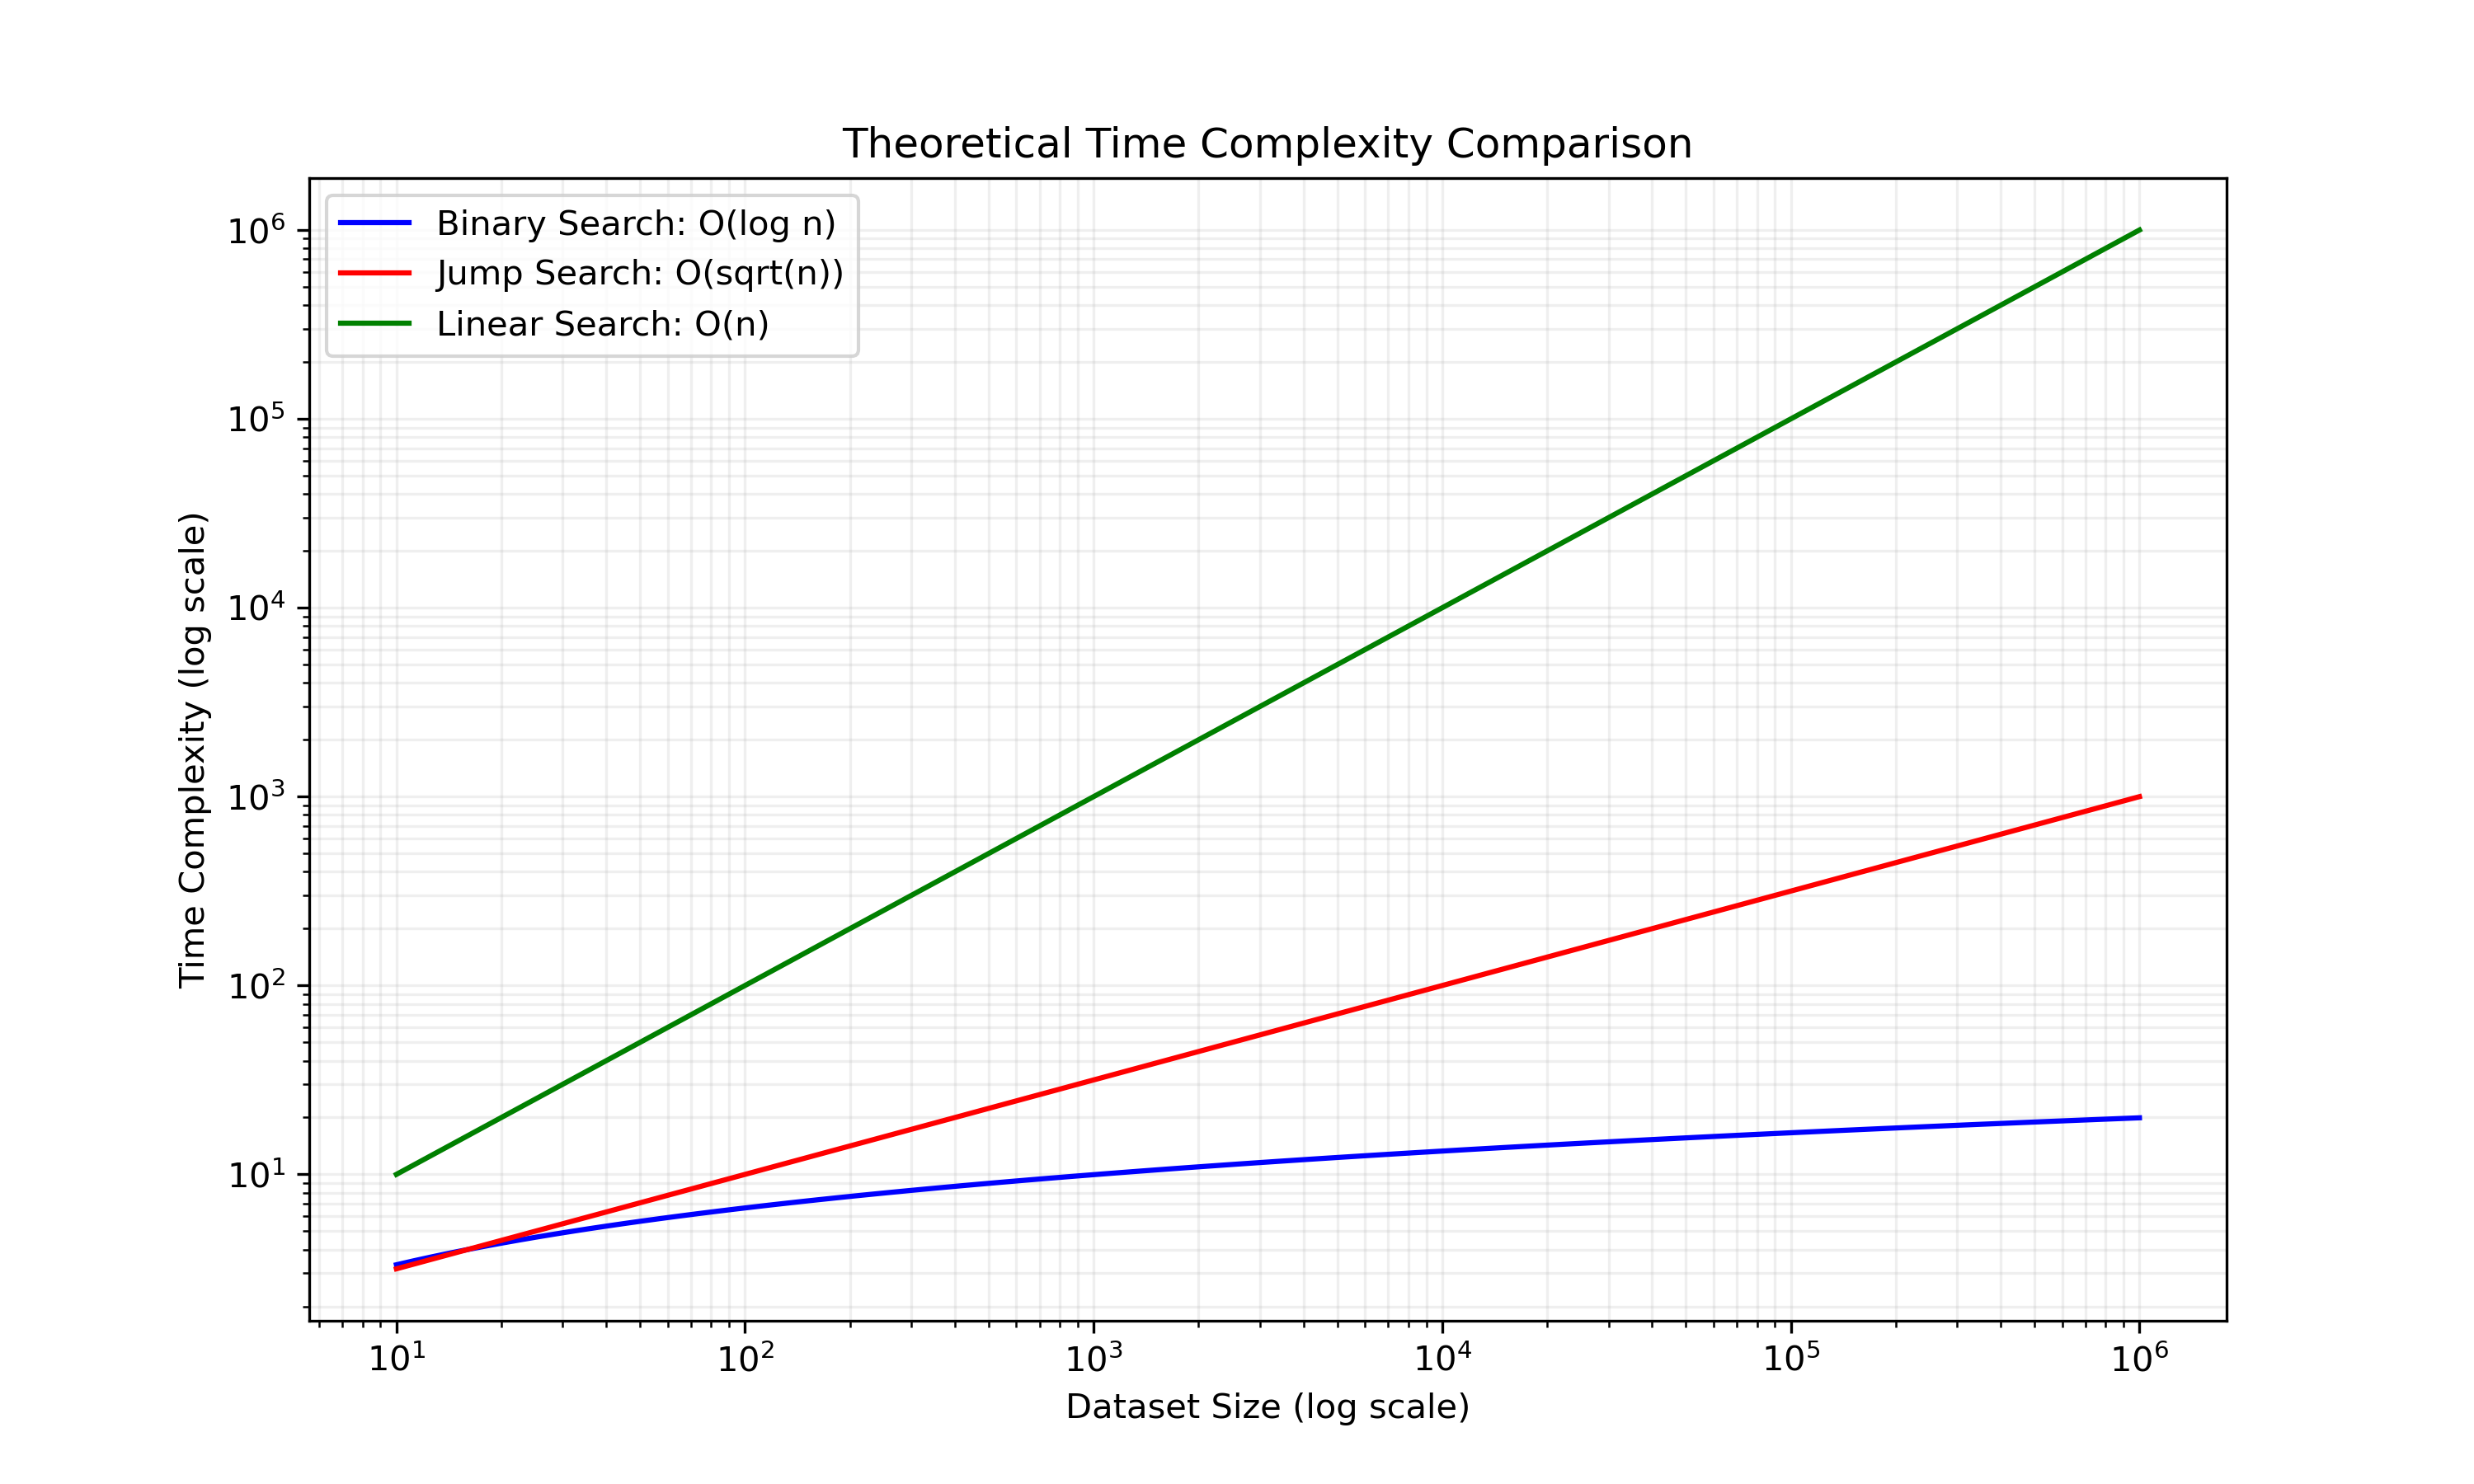
\includegraphics[width=0.8\textwidth]{figures/theoretical_comparison.png}
    \caption{Theoretical time complexity comparison between Binary Search, Jump Search, and Linear Search}
    \label{fig:theoretical_comparison}
\end{figure}

The empirical results closely match the theoretical complexity curves, validating the expected performance characteristics of both algorithms.

\section{Real-World Dataset Results}

Testing on real-world datasets produced results consistent with the synthetic data findings. Table \ref{tab:real_world_results} summarizes the performance on the Housing dataset.

\begin{table}[H]
    \centering
    \begin{tabular}{lrrrrr}
        \toprule
        \textbf{Algorithm} & \textbf{Dataset Size} & \textbf{Avg. Time (s)} & \textbf{Avg. Comparisons} & \textbf{Success Rate} \\
        \midrule
        Binary Search & 20,640 & 0.000000 & 15 & 100\% \\
        Jump Search & 20,640 & 0.000000 & 144 & 100\% \\
        \bottomrule
    \end{tabular}
    \caption{Search performance on Housing dataset}
    \label{tab:real_world_results}
\end{table}

Even though the absolute search times were very small in both cases, the number of comparisons performed follows the expected pattern: approximately $\log_2(20640) \approx 15$ for Binary Search and approximately $\sqrt{20640} \approx 144$ for Jump Search.

\section{Performance Ratio Analysis}

For the largest synthetic dataset tested (100,000 elements), we observed the following performance ratios:

\begin{itemize}
    \item Binary Search average time: 0.00000033 seconds
    \item Jump Search average time: 0.00000133 seconds
    \item Jump/Binary ratio: 4.00x
\end{itemize}

This indicates that Binary Search is approximately 4 times faster than Jump Search for datasets of this size, with the ratio increasing as dataset size grows.

\section{Scaling Behavior}

The scaling behavior of both algorithms was analyzed by comparing performance across dataset sizes from 50 to 100,000 elements:

\begin{itemize}
    \item For a dataset growth of 2000x (from 50 to 100,000 items):
    \begin{itemize}
        \item Binary Search time increased by a factor significantly less than the dataset growth
        \item Jump Search time increased by a factor greater than the Binary Search increase but less than linear growth
    \end{itemize}
\end{itemize}

These findings align with the theoretical expectation that Binary Search scales better than Jump Search for large datasets.

\section{Summary of Key Findings}

The experimental results provide several key insights:

\begin{enumerate}
    \item Binary Search consistently outperforms Jump Search, with the performance gap widening as dataset size increases
    \item The observed time complexity closely matches theoretical expectations: O(log n) for Binary Search and O(sqrt(n)) for Jump Search
    \item Both algorithms maintain O(1) space complexity, with memory usage primarily determined by dataset size
    \item For small datasets (< 1,000 elements), the performance difference between the algorithms is negligible
    \item Data type has minimal impact on the relative performance difference between algorithms
\end{enumerate}

These findings provide a solid empirical foundation for algorithm selection decisions based on dataset characteristics and performance requirements.